% !TeX program = xelatex
% !TEX encoding = UTF-8 Unicode

\documentclass[9pt]{article}
\usepackage{hyperref}
\usepackage{ulem} 
\usepackage{mathtools}
\usepackage{enumitem}
\usepackage{color,soul}
\usepackage{inputenc}
\usepackage[margin=2.75cm]{geometry}
\usepackage{xcolor}
\usepackage{listings}
\usepackage{verbatim}
\usepackage{fancyvrb}
\usepackage{fvextra}

% redefine \VerbatimInput
\RecustomVerbatimCommand{\VerbatimInput}{VerbatimInput}%
{
	fontsize=\small,
	breaklines=true,
	frame=lines,  % top and bottom rule only
	framesep=.75em, % separation between frame and text
	commandchars=\|\(\), % escape character and argument delimiters for commands within the verbatim
	% commentchar=\#        % comment character
	rulecolor=\color{gray},
	%
	%	label=\fbox{\color{Black}data.txt},
	labelposition=topline,
}

\lstset{basicstyle=\ttfamily,
	showstringspaces=false,
	commentstyle=\color{blue},
	keywordstyle=\color{red}
}
\lstset{
	language=bash,
	basicstyle=\ttfamily
}

\begin{document}

\title{Shell Scripting 2020: Week 5}
\author{\textbf{Stefan Ciprian Voinea}\\Student number: 015383372}
\maketitle

%\begin{figure}[h!]
%	\centering
%	\includegraphics[width=12cm]{autoconfiguration.png}
%	\caption{IPv6 Autoconfiguration example}
%	\label{fig:autoconfig}
%\end{figure}

\begin{enumerate}
	
	\setcounter{enumi}{36}
	
	\item \textbf{Counting in the shell}
	
		Contents of the \texttt{task37\_bc\_average.sh} file:
		\VerbatimInput{../task37_bc_average.sh}
	
		Output of the execution:
		\begin{figure}[h!]
			\centering
			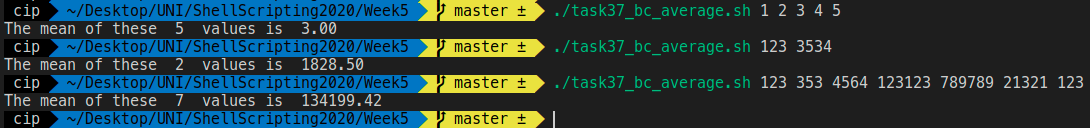
\includegraphics[width=\linewidth]{img/task37.png}
		\end{figure}
		
	
	\item \textbf{Gone in 10 seconds}
	
	\item \textbf{Hipstafy-dropbox}
	
	\item \textbf{Summoning deamons}
	

\end{enumerate}

\end{document}